\chapter{Event Generation and Simulation}
\label{chapter:eventGenSim}

In order to guide an analysis (whether the goal is to search for a new particle
or to measure the strength of a physical coupling), it is important to
understand how the physical aspects will manifest themselves within the context
of the LHC and CMS. For optimizing analysis strategies, physicists utilize an
extensive method of simulation, based on the Monte Carlo
methodology~\cite{MCMethod}. From the interactions between quarks, the
kinematics of intermediate particles, the decay into final products, and the
final interaction of final-state particles with the CMS detector, these
simulations are designed to paint a full picture of the physical event.

\section{Monte Carlo Simulation}
\label{sec:mcSim}
The basis of the simulations lies in the Monte Carlo method, which
uses randomization to sample an integration space and, if numerous enough, will
converge to a known underlying distribution. In this way, it is possible to
create enormous samples of simulated events which follow the underlying
equations governing the fundamental interactions. 

The first step in the simulation process is to calculate the \emph{matrix
element} of an process. The matrix element corresponds to the probability of
some physical process, typically visualized with Feynman diagrams like those
from Chapter~\ref{chapter:sm}.  In order to provide a suitably robust set of
simulation events, events are generated by sampling the matrix element
\emph{phase space} (the allowed kinematic regime of a process). For each point
sampled, a weight is calculated, based roughly on how likely an event in that
region of phasespace would be. Once a full sample is produced, the events are
then `unweighted'. In this process, these weights are normalized to
the maximum value. Then, for each event, a random number is thrown and, if the
random number is larger than the normalized weight, the event is rejected. In
this way, the final collection of events each have an equal weight, but are
composed of a properly distributed population.

Because of the complex structure of the collisions at the LHC, it is impossible to
measure (and tune) the momenta of the constituents involved in the processes. As
a result, these matrix elements are also dependent on the \emph{parton
distribution functions} (PDFs). These are probabilistic functions which define
the relative amounts of momentum carried by each of the constituents in the
protons involved in the collision. Due to the energy scales of the interactions
involved, these probabilities are beyond the scope of current QCD calculations,
so as a result, the PDFs are derived based on previous experimental probings of
the partonic structure~\cite{MSTW08,ct10,nnPDF}. A comparison of the three PDF
sets used within this analysis is shown in Figure~\ref{fig:pdfComp}, reproduced
from~\cite{pdfComp}.

\begin{figure}[h]
\centering
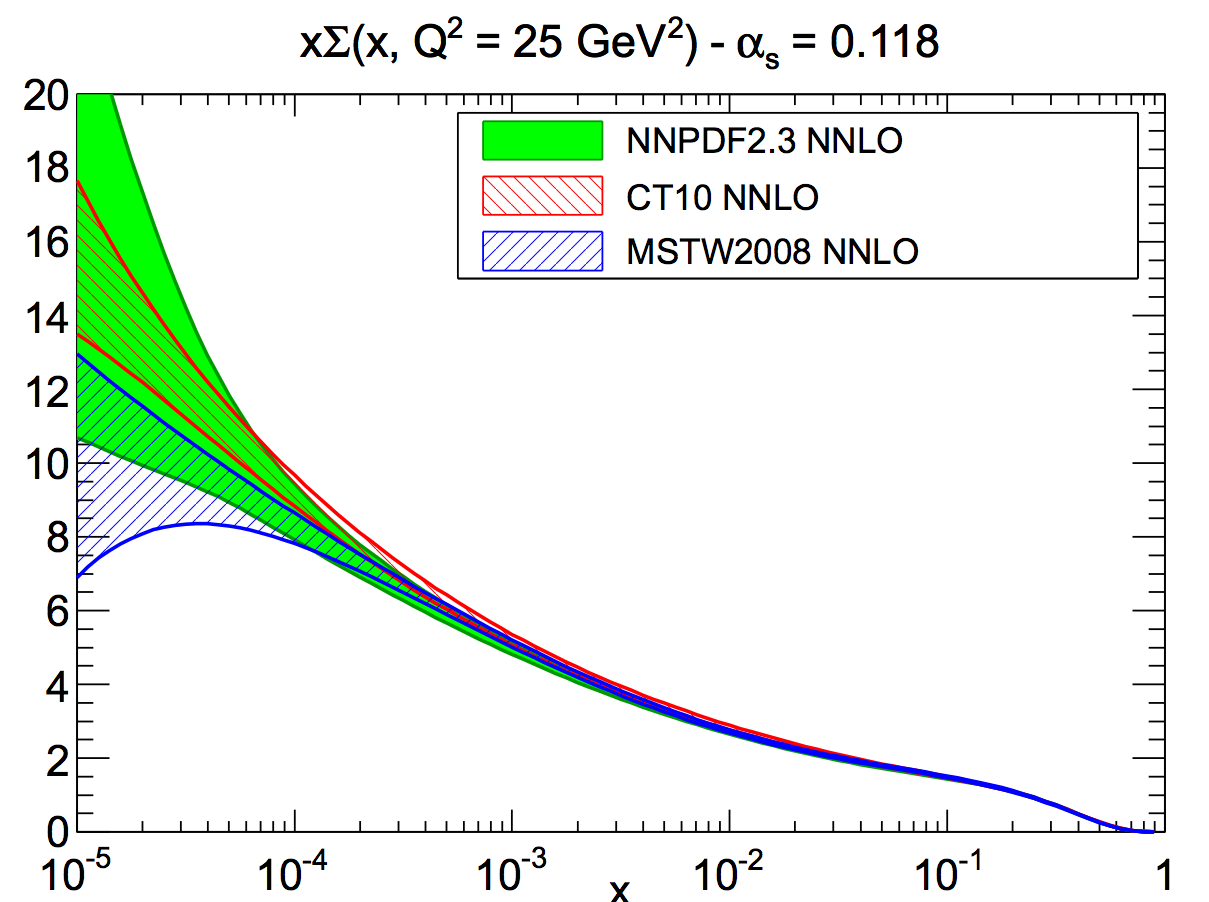
\includegraphics[width=0.80\textwidth]{pdfComp}
\caption[A comparison of three different PDF sets.]{A comparison of the PDF sets NNPDF~\cite{nnPDF}, CT10~\cite{ct10}, and
MSTW08~\cite{MSTW08}, reproduced from~\cite{pdfComp}.}
\label{fig:pdfComp}
\end{figure}

\section{Parton Showering} 
Although the matrix element method outlined in Section~\ref{sec:mcSim} simulates
the hard (high-momentum transfer) of event, it does not provide any simulation
of any of the hadronic showering in the event. As mentioned in
Chapter~\ref{chapter:sm}, individual partons cannot be observed, instead
forming a cascade of hadrons which shower the detector. This hadronic activity
can arise through the hard interactions directly (for example, a \Z boson
decaying hadronically), radiated from an initial or final state, or from the
\emph{underlying event}. The underlying event is a result of QCD's color
conservation--as the partons in the proton interact in the hard process, the
partons that remain in the proton must themselves form into colorless states.

Because of the low energies involved in the soft interactions, it is difficult
(or impossible) to apply the standard tools of QCD calculations to the
hadronization process. Instead, a purely phenomenological approach is taken,
known as the Lund string model~\cite{lundStringModel}. In this model, the partons are
attached with a gluon `string'. As the string stretches (meaning the partons
move apart), its energy increases until it can create new quark/antiquark
pairs, at which point it `snaps'. Quarks and antiquarks from nearby sprays can
combine into mesons, or the quark cascade can continue, as diagrammed in
Fig.~\ref{fig:hadronization}.

\begin{figure}[h]
\centering
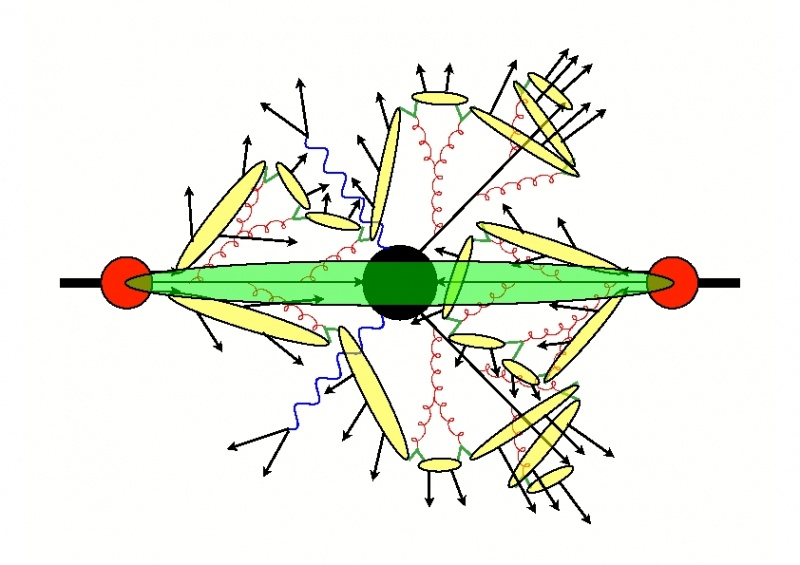
\includegraphics[width=0.80\textwidth]{hadronization}
\caption[Diagrammatic representation of a hadronization process.]{A diagram
depicting the hadronization process\cite{hadronization}. The hard process is
highlighted in green, while the various hadronizations are in yellow.}
\label{fig:hadronization}
\end{figure}

\section{Pile-up}
In addition to the simulation of the hard process and the partonic showering,
simulated physics events also require a description of the \emph{pile-up}.
Pile-up events are interactions which occur between other protons within the
bunch crossing. In order to simulate the effect that these events have on the
hard process, \emph{minimum bias} (soft events) are superimposed on top of the
event of interest. The number of these events added is assigned randomly so that
the overall distribution of the amount of pileup per event matches the data as
closely as possible. Because of the long timeline involved in generating MC
samples, it is necessary to apply corrections in order to properly represent the
distribution in data. These corrections are further explained in
Chapter~\ref{chapter:analysis}).

%\begin{figure}[h]
%\centering
%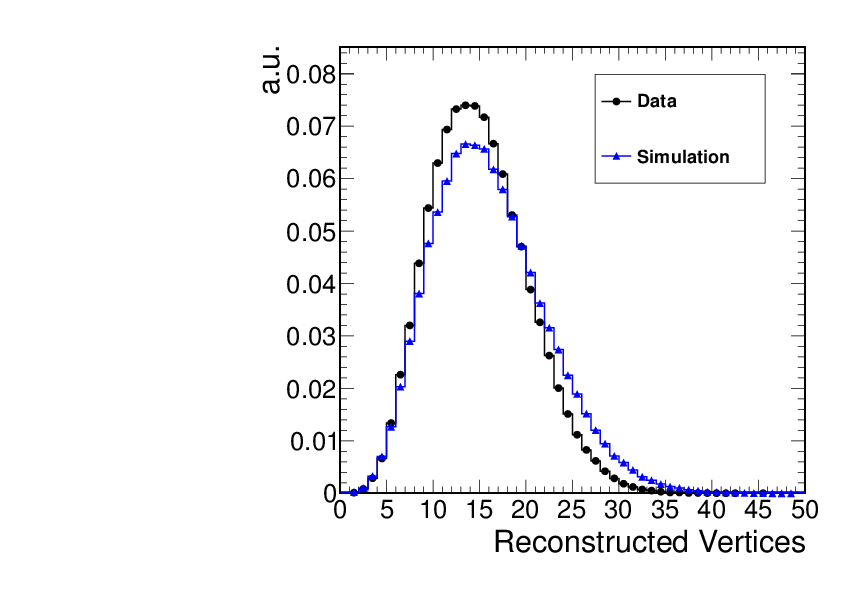
\includegraphics[width=0.80\textwidth]{compvertices}
%\caption[Comparison of data and uncorrected simulated pile-up distributions.]{An example comparison between the simulated number of reconstructed
%vertices (blue triangles) and the final distribution seen in data (black dots).
%The differences are accounted for via corrections explained in
%Chapter~\ref{chapter:analysis}.}
%\label{fig:vertices}
%\end{figure}

\section{Generator Software}

There are many different software packages that have been written for MC event
generation. They primarily differ in the order of the calculation. Some, such as
Sherpa and Pythia, involve only leading order perturbative QCD calculations.
Other generators, such as POWHEG BOX, MADGRAPH, MC@NLO, and MCFM include
next-order effects in the calculations. Typically, the LO MC generators include
the full chain from initial state to final detectable objects. The NLO
generators, are typically interfaced with a second program (commonly PYTHIA) in
order to handle the hadron showering processes.

\section{Samples used}
This analysis utilizes both NLO and LO matrix element generators, while relying
on Pythia~\cite{PYTHIA} for all showering, hadronization, and underlying event
generation.

The primary Higgs boson signal samples are generated using POWHEG~\cite{POWHEG},
covering both the gluon-gluon fusion and vector boson fusion production
mechanisms at NLO. These samples are weighted to NNLO calculations (VBF) or
NNLO+NNLL (gg) (\cite{yellowReport}). Although the generated Higgs $p_T$ spectra
does not match that of the NLO+NNLL calculations, the effects of this difference
were found to be negligible to the analysis as a whole.

Two different matrix element generators are used in production of the Standard
Model ZZ samples. $q\overline q \rightarrow ZZ \rightarrow \ell\ell\ell\ell$
samples are produced with POWHEG at NLO, while $gg\rightarrow ZZ$ production is
handled at LO via gg2zz~\cite{gg2zz}.

Samples with anomalous triple gauge couplings were all produced with
the LO generator SHERPA~\cite{SHERPA}, as it is the only ME generator which has
the requisite couplings modelled. Although only a LO generator, an extensive
study indicated that the generator well reproduces the four-lepton invariant
mass 

MADGRAPH~\cite{MADGRAPH} is used to produce the simulated sample of
$\Z\rightarrow \ell\ell$ plus hadronic jet activity, which is the largest
reducible background. The use of MADGRAPH in these samples is important, as the
accurate modelling of the jets is especially critical, given that this
background enters the signal region through the hadronic jets faking a
signal-like lepton. This sample is weighted to the calculated NNLO cross
section.

More specific information about the samples used in this analysis are in
Tables~\ref{tab:MC_samples}.

\begin{sidewaystable}
\small
\centering
\begin{tabular}{|c|c|c|c|}
\hline

%\multicolumn{4}{|c|}{7 TeV Samples} \\ 
%\hline
%Sample & Generator & $\sigma$ (pb) & Notes\\
%\hline
%
%ZZTo4[l]\_mll4\_7TeV-powheg-pythia6/Fall11& POWHEG & 0.06609 & $m_{\ell\ell} > 4
%GeV$, l=e,mu,tau\\
%ZZTo2[l]2[l']\_mll4\_7TeV-powheg-pythia6/Fall11& POWHEG & 0.152 & $m{\ell\ell} > 4
%GeV$, l, l'=e,mu,tau \\
%GluGluToZZTo4L\_7TeV-gg2zz-pythia6/Fall11& gg2zz & 0.00174 & \\
%GluGluToZZTo2L2L\_7TeV-gg2zz-pythia6/Fall11 & gg2zz & 0.00348 & \\
%DYJetsToLL\_TuneZ2\_M-50\_7TeV-madgraph-tauola & MADGRAPH & 3048 & $m{\ell\ell} >
%4$\\
%
%GluGluToHToZZTo4L\_M-*\_7TeV-powheg-pythia6/Fall11 & POWHEG & * & \\
%VBF\_HToZZTo4L\_M-*\_7TeV-powheg-pythia6/Fall11 & POWHEG & * & \\
%WH\_ZH\_TTH\_HToZZ\_M-*\_7TeV-pythia6/Fall11 & POWHEG & * & \\
%ZZTo4L with aTGCs & SHERPA & 0.046-0.098** & $m_{\ell\ell} > 12 GeV$, e/$\mu$
%only \\
%
%\hline

\hline
\multicolumn{4}{|c|}{8 TeV Samples} \\ 
\hline
Sample & Generator & $\sigma$ (pb) & Fiducial cuts \\
\hline
ZZTo4[l]\_8TeV-powheg-pythia6/Summer12 & POWHEG & 0.07691 & $m_{\ell\ell} > 4
GeV$, l=e,mu,tau \\
ZZTo2[l]2[l']\_8TeV-powheg-pythia6/Summer12 & POWHEG & 0.1767 & $m_{\ell\ell} > 4
GeV$, l, l'=e,mu,tau \\
GluGluToZZTo4L\_8TeV-gg2zz-pythia6/Summer12 & gg2zz & 0.0048 & $m_{\ell\ell} >
4 GeV$\\
GluGluToZZTo2L2L\_TuneZ2star\_8TeV-gg2zz-pythia6/Summer12 & gg2zz & 0.01208 &
$m_{\ell\ell} < 4 GeV$ \\
DYJetsToLL\_M-50\_TuneZ2Star\_8TeV-madgraph-tarball/Summer12 & MADGRAPH &
3503.71 & $m{\ell\ell} > 50 GeV$ \\
DYJetsToLL\_M-10To50filter\_8TeV-madgraph/Summer12 & MADGRAPH & 915 & $10 <
m_{\ell\ell} < 50 GeV$ \\
TTTo2L2Nu2B\_8TeV-powheg-pythia6/Summer12 & POWHEG & 23.64 & \\

GluGluToHToZZTo4L\_M-*\_8TeV-powheg-pythia6/Summer12 & POWHEG & * & \\
VBF\_HToZZTo4L\_M-*\_8TeV-powheg-pythia6/Summer12 & POWHEG & * & \\
WH\_ZH\_TTH\_HToZZ\_M-*\_8TeV-pythia6/Summer12 & POWHEG & * & \\
ZZTo4L with aTGCs & SHERPA & 0.057-0.064** & $m_{\ell\ell} > 12 GeV$, e/$\mu$
only \\

\hline
\end{tabular}
\caption[Summary of Monte Carlo samples used.]{A list of the samples utilized in the 8
TeV portion of this analysis, the generator used, and the sample cross-section.
A * denotes the fact that there was a wide range of Higgs masses used, while a
** means that there was a number of different coupling values used. Full details
for each are explained in Chapter~\ref{chapter:analysis}.}
\label{tab:MC_samples}
\end{sidewaystable}


\section{Detector Simulation}
Once the physics events are generated, their interactions with the material
composing CMS (and their resulting detection) must also be simulated via
GEANT4~\cite{GEANT4}. At its core, this software suite simulates the stochastic
interactions between the particles created in the collision and the matter of
CMS (both detecting and non-detecting). GEANT4 contains an in-depth geometrical
model of CMS, from the specifications of the detecting components to the material
budget of the non-detecting portions (such as structural support and readout
electronics). GEANT4 also provides simulation of the effects of the solenoid,
calculating trajectories based on actual magnetic field measurements. 

GEANT4 provides a picture of how the particles interact with the detector
components, but one final stage remains in the event simulation chain. In order
to be fully comparable to experimental data, the events must pass through a
simulated version of the electronic detector readout. Each subcomponent of the
detector provides an electronics simulation, so that effects of electronic noise
and timing are represented in the simulated samples. At the end of this
simulation chain, the MC samples exist in the same raw format as the data when
read out by the CMS detector. As a result, both simulation and real data can be
passed through the same \emph{reconstruction} process, allowing direct
head-to-head comparisons between the two.
